\documentclass[12pt]{beamer}

% ****************
% ***** INFO *****
% ****************
\usepackage[english]{babel}
\title[Insitute]{Analysis of Inter-LLM and Intra-LLM Alignment in Image Description and Generation}
\subtitle{Assets for \LaTeX}
\author[Name Surname]{Saverio Napolitano}
\institute[]{Mid Sweden University}
\newcommand{\course}{Quantitative Research and Development}
\newcommand{\currentyear}{\the\year} % \currentyear
\newcommand{\nextyear}{\the\numexpr\year+1\relax} % \nextyear
\date{\currentyear/\nextyear} % or \today

% *******************
% ***** PROJECT *****
% *******************
\definecolor{main}{HTML}{0000FF}
\setbeamercolor{structure}{fg=main}

% *****************
% ***** THEME *****
% *****************
\usetheme{Luebeck}
\usepackage{helvet}
\renewcommand{\familydefault}{\sfdefault}
\setbeamertemplate{frametitle continuation}{\gdef\beamer@frametitle{}}
\setbeamertemplate{footline}{}

% *****************
% ***** CODE *****
% *****************
\usepackage{listings}
\usepackage[export]{adjustbox}
\lstdefinestyle{java}{
    backgroundcolor=\color{white},
    basicstyle=\ttfamily\scriptsize,
    breaklines=true,
    commentstyle=\color{gray},
    keywordstyle=\color{blue},
    stringstyle=\color{magenta},
    identifierstyle=\color{black},
    numberstyle=\color{gray},
    language=Java
}
\lstdefinestyle{cpp}{
    backgroundcolor=\color{white},
    basicstyle=\ttfamily\scriptsize,
    breaklines=true,
    commentstyle=\color{gray},
    keywordstyle=\color{blue},
    stringstyle=\color{magenta},
    identifierstyle=\color{black},
    numberstyle=\color{gray},
    language=C++
}
\lstdefinestyle{py}{
    backgroundcolor=\color{white},
    basicstyle=\ttfamily\scriptsize,
    breaklines=true,
    commentstyle=\color{gray},
    keywordstyle=\color{blue},
    stringstyle=\color{magenta},
    language=Python
}
\lstdefinestyle{js}{
    backgroundcolor=\color{white},
    basicstyle=\ttfamily\scriptsize,
    breaklines=true,
    commentstyle=\color{gray},
    keywordstyle=\color{blue},
    stringstyle=\color{magenta},
    identifierstyle=\color{black},
    numberstyle=\color{gray},
    language=JavaScript,
    escapechar=@
}
\lstdefinestyle{sh}{
    basicstyle=\ttfamily\scriptsize,
    breaklines=true,
    commentstyle=\color{gray},
    keywordstyle=\color{blue},
    stringstyle=\color{magenta},
    identifierstyle=\color{black},
    numberstyle=\color{gray},
    language=bash
}

% **********************
% ***** ALGORITHMS *****
% **********************
\usepackage{algorithm}
\usepackage{algpseudocode}

% *****************
% ***** UTILS *****
% *****************
\usepackage{xcolor}

% ********************
% ***** DOCUMENT *****
% ********************
\begin{document}

% **********************
% ***** TITLEPAGE ******
% **********************
\begin{frame}{}
%\vspace{\fill}

%\includegraphics[width=0.16\linewidth]{example-image}

\vspace{\fill}

\Large
\color{main}
\inserttitle

\medskip

\large
\color{black}
%\insertsubtitle

\vspace{\fill}

\footnotesize
\insertinstitute

\footnotesize
\course


\vspace{\fill}

\textbf{Author:} \insertauthor

\medskip

\insertdate

\vspace{\fill}
\end{frame}

% *****************
% ***** START *****
% *****************
\begin{frame}[allowframebreaks]{Outline}
\begin{itemize}
    \item Transformer 
    \begin{itemize}
        \item Attention
    \end{itemize} 
    \item Large Language Model (LLM)
    \begin{itemize}
        \item Multimodal Large Language Model 
        \begin{itemize} 
            \item Contrastive Image-Language Pre-training (CLIP)
        \end{itemize}
        \item Large Language Model for Image Captioning 
        \item Large Language Model for Image Generation 
    \end{itemize}
\end{itemize}
\end{frame} 

\begin{frame}[allowframebreaks]{Transformer}
    \begin{figure}
        \centering
        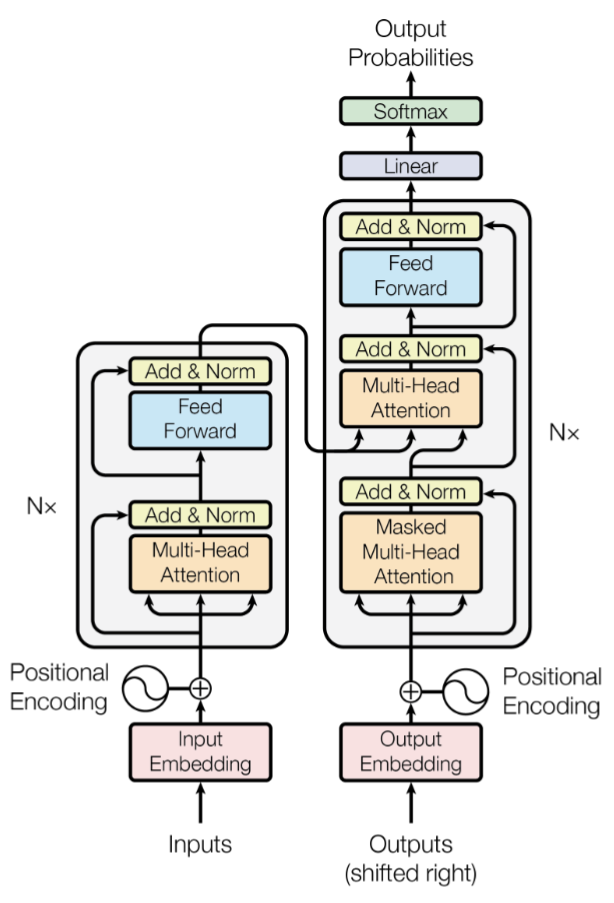
\includegraphics[height=0.6\textheight]{figures/transformer_architecture.png}
        \caption{The Transformer - model architecture. Reprinted from Figure 1 in Vaswani et al. (2017)~\cite{vaswani2017attention}.}
        \label{fig:Fig. 1}
    \end{figure}
\end{frame}

\begin{frame}[allowframebreaks]{Attention}
    \begin{figure}
        \centering
        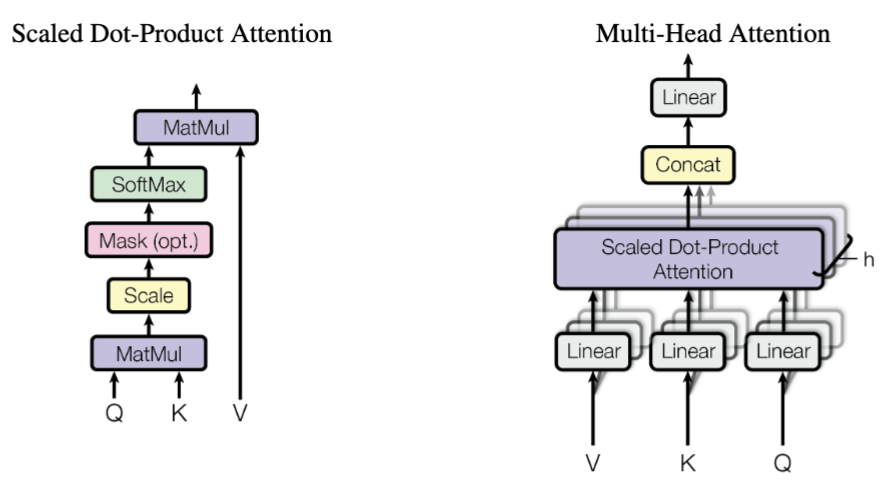
\includegraphics[height=0.6\textheight]{figures/attention.png}
        \caption{(left) Scaled Dot-Product Attention (right) Multi-Head Attention consists of several attention layers running in parallel. Reprinted from Figure 2 in Vaswani et al. (2017)~\cite{vaswani2017attention}.}
        \label{fig:Fig. 2}
    \end{figure}
\end{frame}

\begin{frame}[allowframebreaks]{Large Language Model (LLM)}
    \begin{figure}
        \centering
        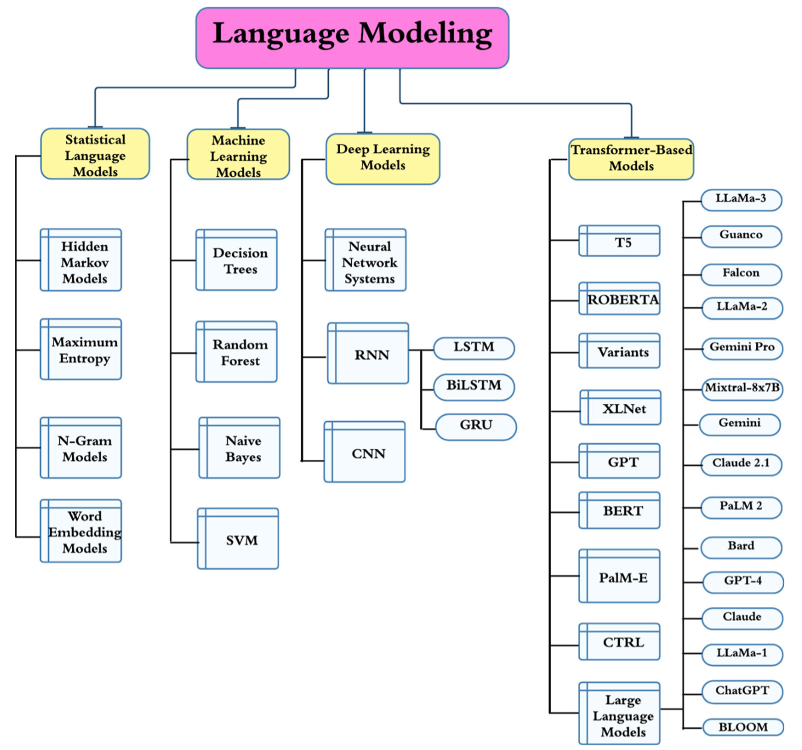
\includegraphics[height=0.6\textheight]{figures/lm_taxonomy.png}
        \caption{Types of language modeling. Reprinted from Figure 1 in Hadi et al. (2025)~\cite{Hadi_2025}.}
        \label{fig:Fig. 3}
    \end{figure}
\end{frame}

\begin{frame}[allowframebreaks]{Large Language Model (LLM)}
    \begin{figure}
        \centering
        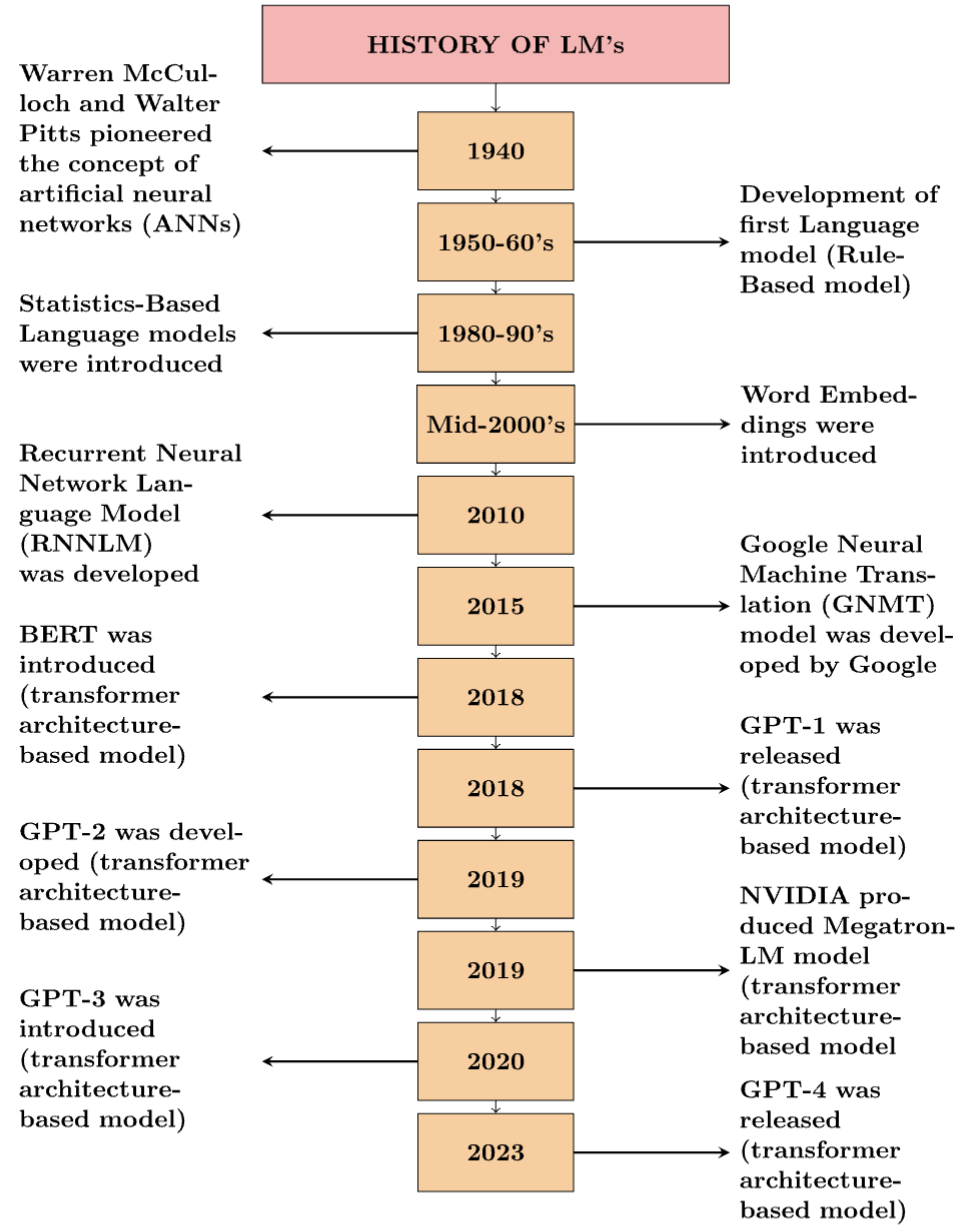
\includegraphics[height=0.6\textheight]{figures/lm_history.png}
        \caption{Brief history of language modeling. Reprinted from Figure 3 in Annepaka et al. (2025)~\cite{Annepaka2025}.}
        \label{fig:Fig. 4}
    \end{figure}
\end{frame}

\begin{frame}[allowframebreaks]{Large Language Model (LLM)}
    \begin{figure}
        \centering
        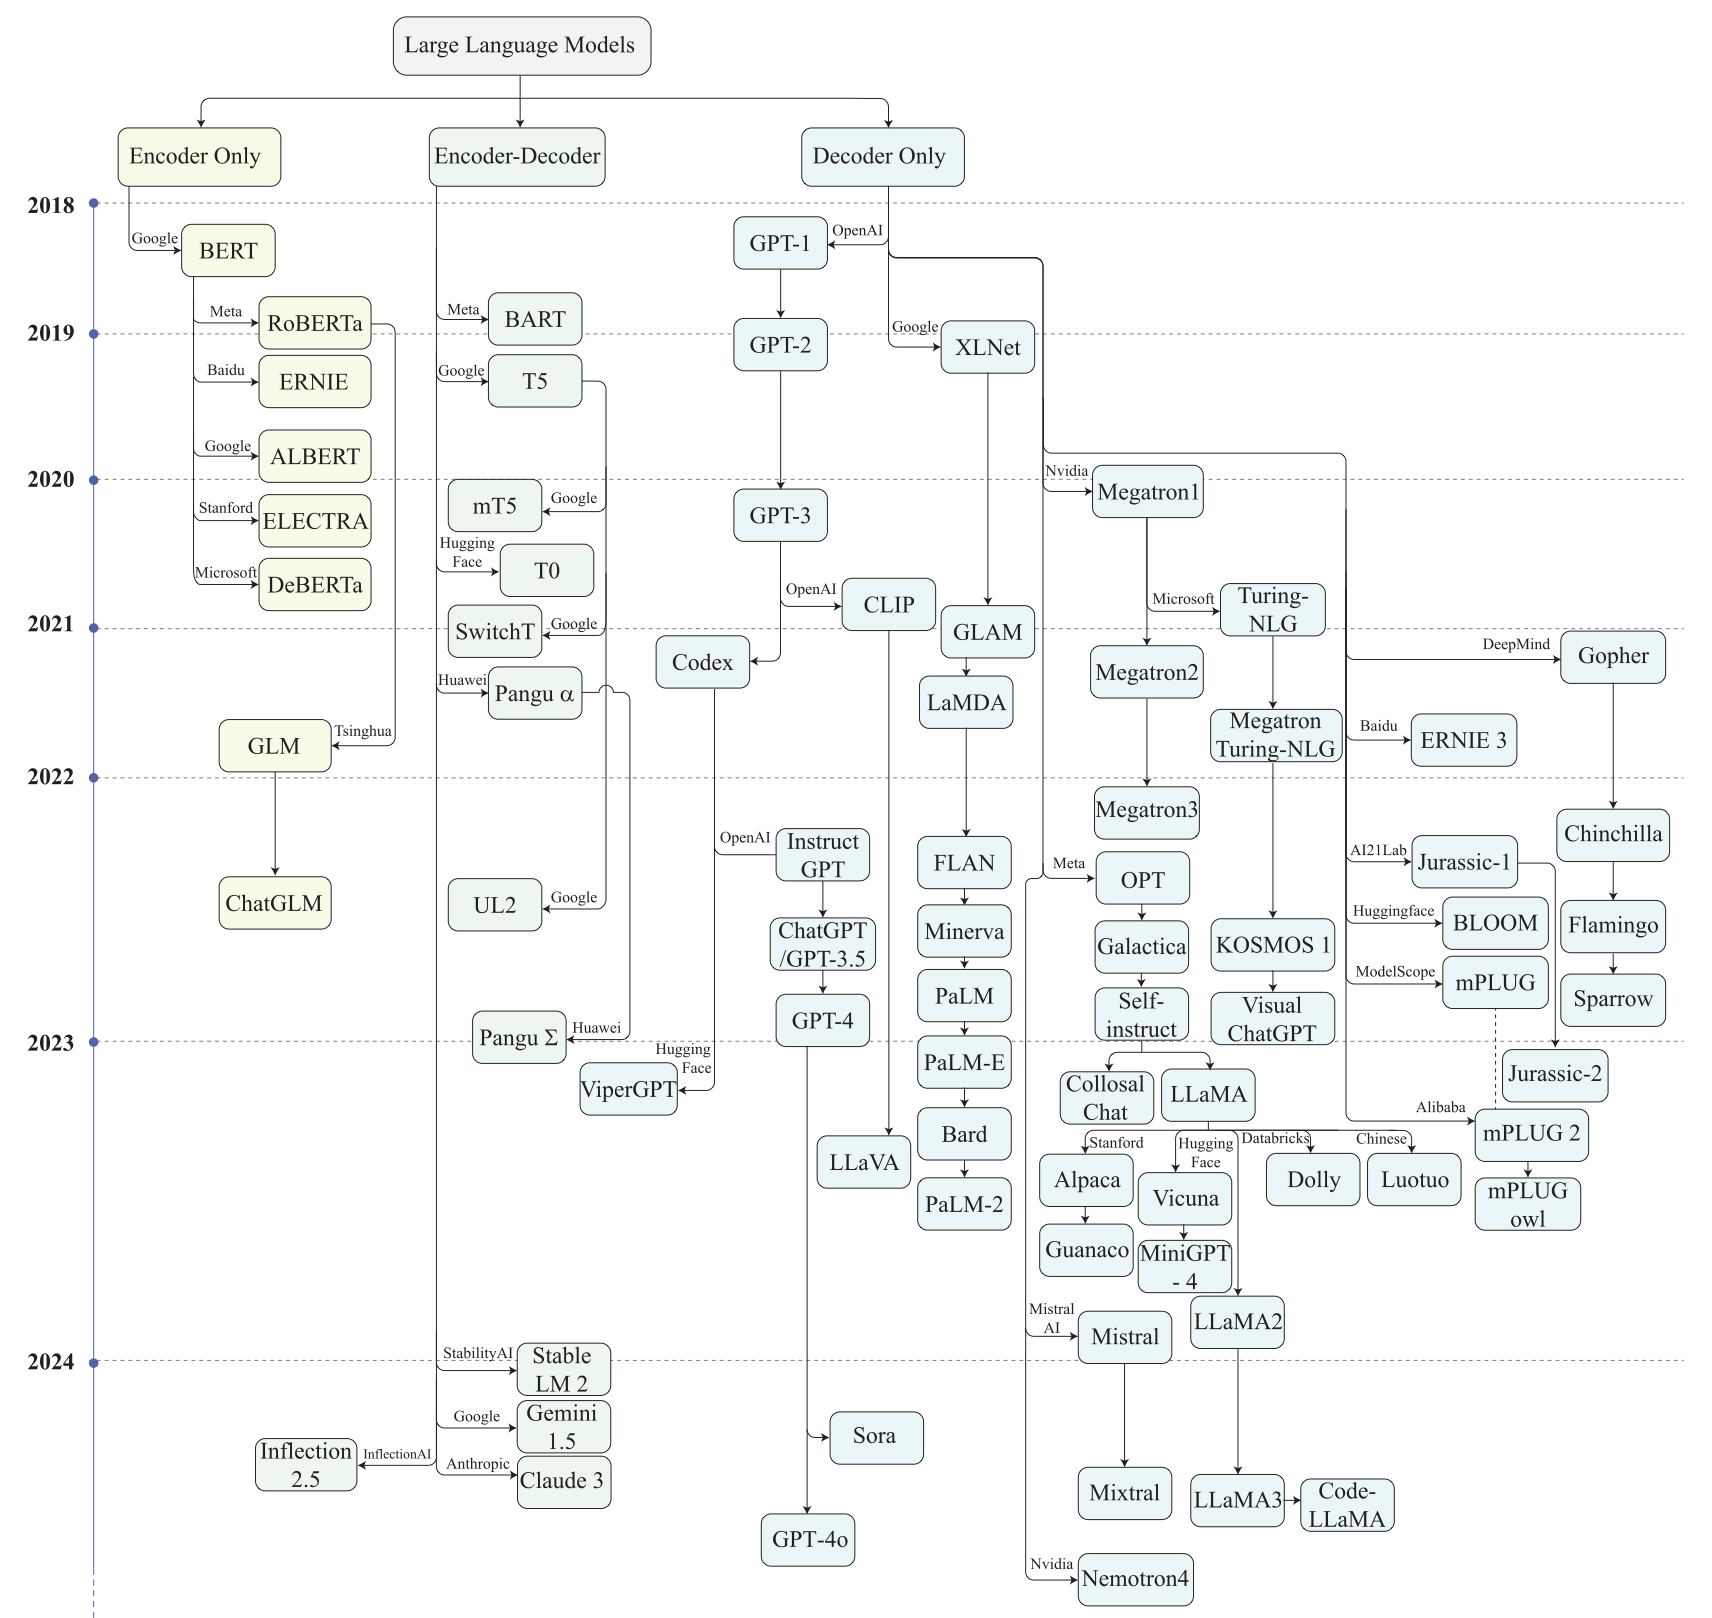
\includegraphics[height=0.6\textheight]{figures/llm_evolution.png}
        \caption{Evolutionary tree illustrating the progression of mainstream LLMs. Reprinted from Figure 12 in Shao et al. (2024)~\cite{10720163}.}
        \label{fig:Fig. 5}
    \end{figure}
\end{frame}

\begin{frame}[allowframebreaks]{Large Language Model (LLM)}
    \begin{figure}
        \centering
        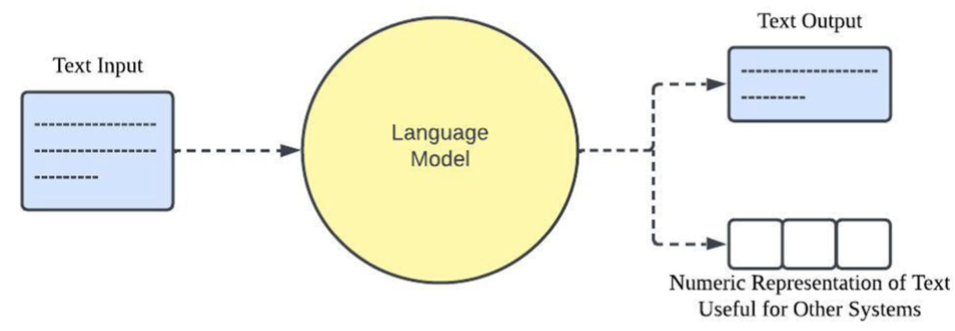
\includegraphics[width=0.9\linewidth]{figures/lm_workflow.png}
        \caption{Workflow of a language model. Reprinted from Figure 2 in Annepaka et al. (2025)~\cite{Annepaka2025}.}
        \label{fig:Fig. 6}
    \end{figure}
\end{frame} 

\begin{frame}[allowframebreaks]{Multimodal Large Language Model}
    \begin{figure}
        \centering
        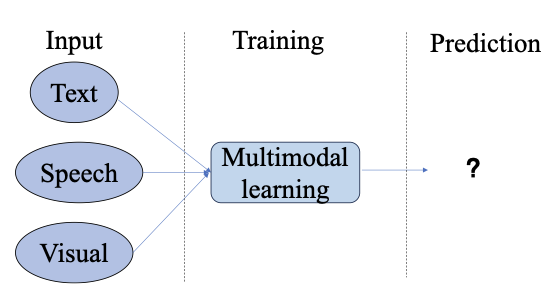
\includegraphics[width=0.9\linewidth]{figures/multimodal_definition.png}
        \caption{Definition of multimodal. Reprinted from Figure 1 in Wu et al. (2023)~\cite{10386743}.}
        \label{fig:Fig. 7}
    \end{figure}
\end{frame}

\begin{frame}[allowframebreaks]{Contrastive Language Image Pre-training (CLIP)}
    \begin{figure}
        \centering
        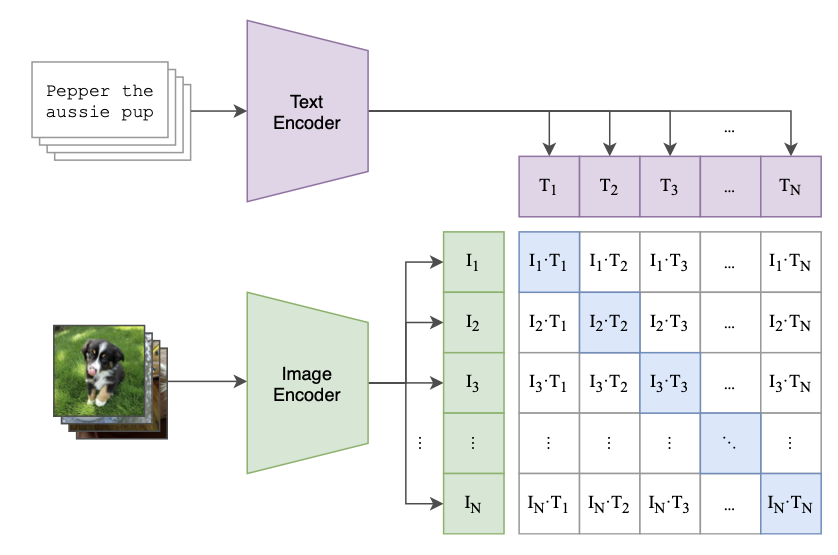
\includegraphics[height=0.5\textheight]{figures/clip.png}
        \caption{CLIP architecture and training. Reprinted from Figure 1 in Radford et al. (2021)~\cite{pmlr-v139-radford21a}.}
        \label{fig:Fig. 8}
    \end{figure}
\end{frame}

\begin{frame}[allowframebreaks]{Large Language Model for Image Captioning}
    \begin{figure}
        \centering
        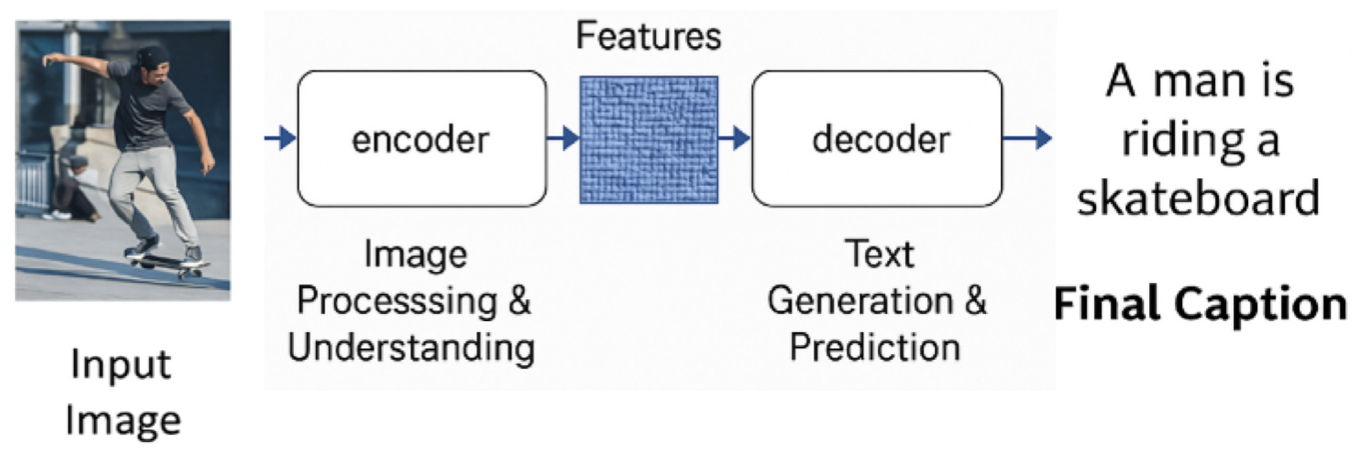
\includegraphics[width=0.9\linewidth]{figures/image_captioning.png}
        \caption{The general structure framework for image captioning. Reprinted from Figure 1 in Abdulgalil et al. (2025)~\cite{ABDULGALIL2025100159}.}
        \label{fig:Fig. 9}
    \end{figure}
\end{frame}

\begin{frame}[allowframebreaks]{Large Language Model for Image Captioning}
    \begin{figure}
        \centering
        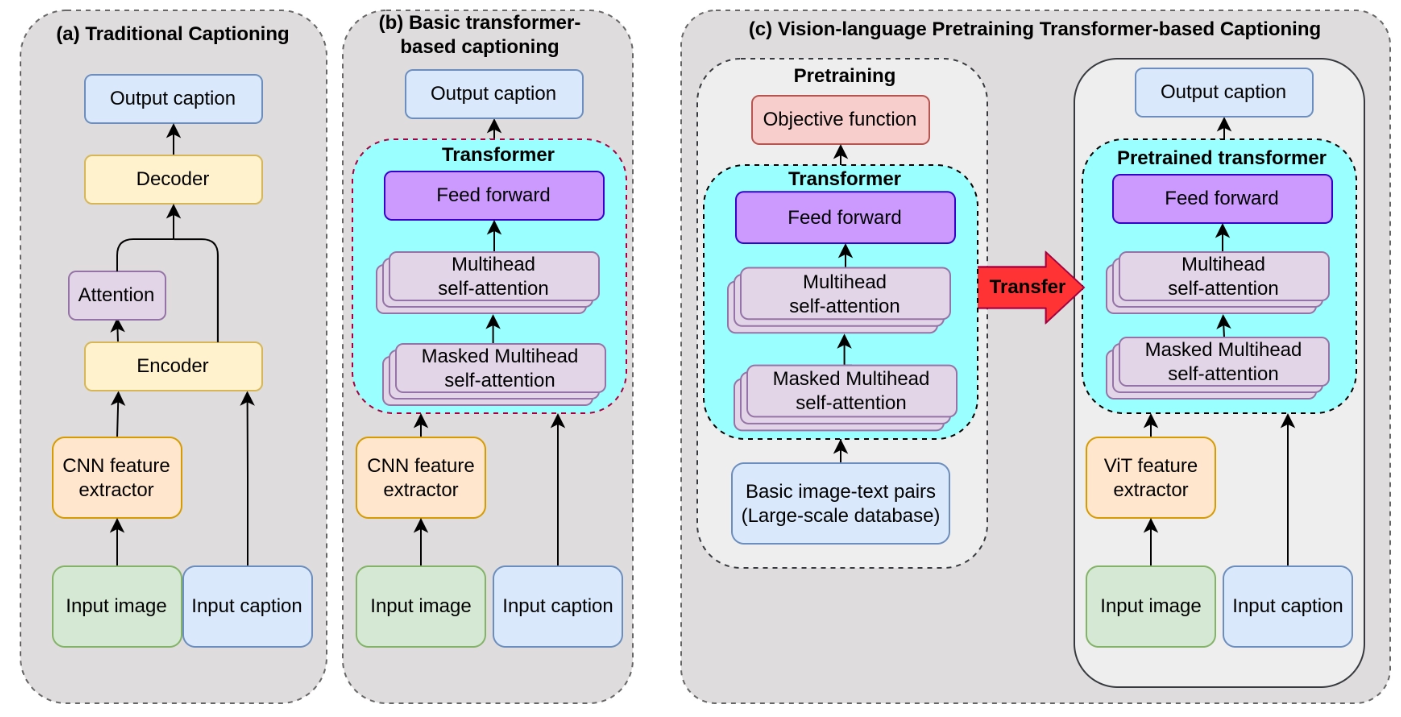
\includegraphics[width=0.9\linewidth]{figures/transformer_image_captioning.png}
        \caption{Development of captioning structures and systems. Reprinted from Figure 1 in Ondeng et al. (2023)~\cite{app131911103}.}
        \label{fig:Fig. 10}
    \end{figure}
\end{frame}

\begin{frame}[allowframebreaks]{Large Language Model for Image Generation}
    \begin{figure}
        \centering
        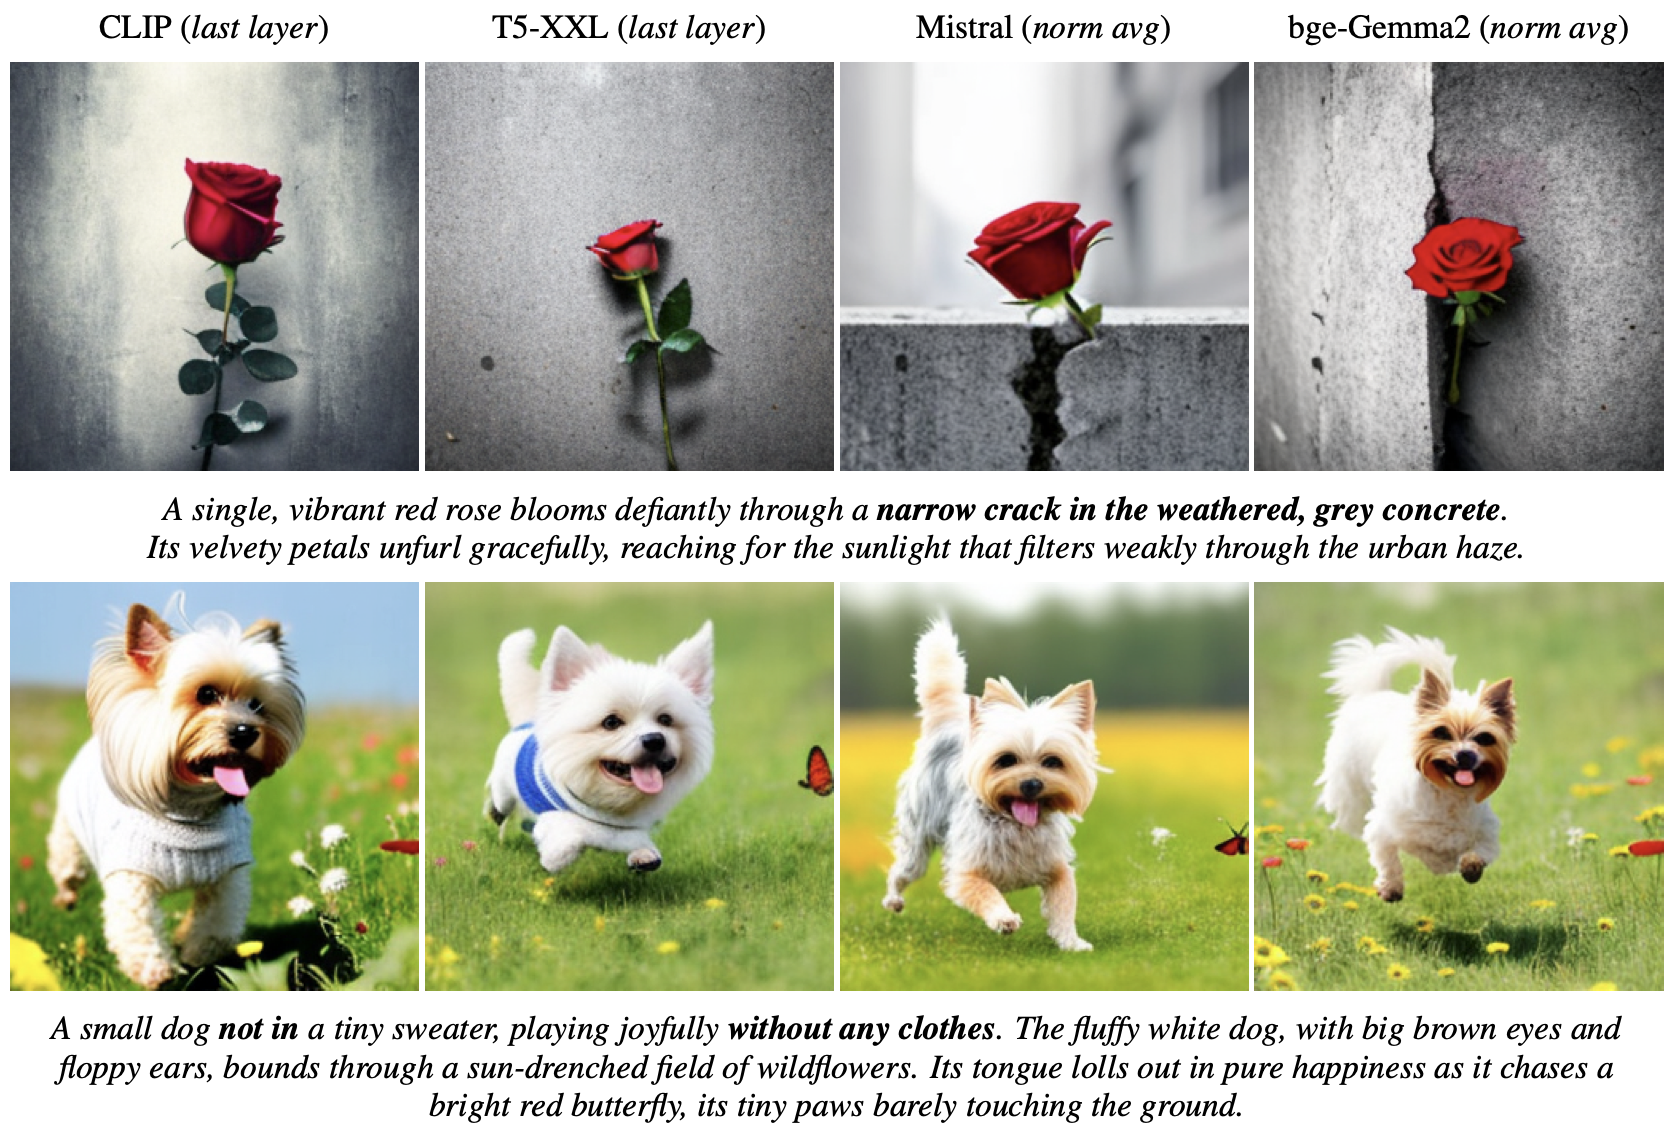
\includegraphics[width=0.9\linewidth, height=0.5\textheight]{figures/image_generation.png}
        \caption{Visual comparison of images generated with different text encoders. Reprinted from Figure 1 in Wang et al. (2025)~\cite{11094992}.}
        \label{fig:Fig. 11}
    \end{figure}
\end{frame}


% ************************
% ***** BIBLIOGRAPHY *****
% ************************
\begin{frame}[allowframebreaks]{Bibliography}

\scriptsize
\bibliographystyle{unsrt}
\bibliography{bib/references}
\end{frame}
% ***************
% ***** END *****
% ***************

\end{document}